\documentclass[a4paper]{article}

\usepackage[english]{babel}
\usepackage[utf8]{inputenc}
\usepackage{amsmath}
\usepackage{graphicx}
\usepackage{subfigure}
\usepackage{hyperref}

\title{Genetic Algorithm for Solving the Multidimensional 0-1 Knapsack Problem}

\author{Simon Kessler}

\date{\today}

\begin{document}
\maketitle

\begin{abstract}

The goal was to design and implement a population based algorithm which is able to solve a multidimensional 0-1 knapsack problem. Best results for the benchmark \emph{mknapcb1} have been obtained by using an initial random population, uniform-crossover and replace-worst strategy. Additional a mutation is applied to each offspring chromosome.

It has been shown, that the crossover probability and the number of worst chromosome replaced has the biggest impact on the quality of the fittest solution.

Finally it has been outlined, that by using the Dantzig algorithm for the initial population and a penalty function for infeasible solutions the quality and speed could be improved.
\end{abstract}

\section{Introduction}

In this paper the design and implementation of a genetic algorithm which can solve the multidimensional 0-1 knapsack problem is presented. Also a discussion about the impacts of various parameters of the algorithm on the quality and computation time of the obtained solution. To benchmark the algorithm the \emph{mknapcb1} file of the OR-Library\footnote{http://people.brunel.ac.uk/~mastjjb/jeb/orlib/mknapinfo.html} is used. Additionally an external paper will be reviewed, to show which modules of the algorithm could be improved by using advanced techniques.

\section{Algorithm Design}

\subsection{Problem Representation}

For a genetic algorithm it is favourable to represent the problem as a bit string, i.e. \emph{01001}, in which each bit represents the state of an item.

\subsection{Modules}

\paragraph{Population} 

To allow a good exploration of the search space, it is important to generate a well distributed initial population. Every chromosome of the population should have for every bit the same probability of 0.5 to be packed in or not. The problem size must be less than or equal \(2^n\) (n = number of items), otherwise it is impossible to create a population due to the following restrictions.

To ensure great diversity a population is not allowed to contain twice the same chromosome. Additionally only valid solutions, that is solutions not breaking any knapsack size constraint are contained. By replacing only a number of the worst chromosomes (\emph{replace-worst}) the chance of replacing a very good chromosome is low. This way good solutions are not prematurely replaced.

\paragraph{Evaluation}

For the knapsack problem the evaluation is straightforward: Sum up the values of each packed item. The total sum is the evaluated value of the solution. If any constraint is broken, a value of -1 is assigned. 

\paragraph{Reproduction}

For assigning the fitness values the strategy \emph{fitness-is-evaluation} is used. The selection of the parents is based on their fitness by using the \emph{roulette-wheel} strategy. However, there is still some probability involved. This is important, as less fit chromosomes still may have some very good parts which are required to obtain an optimal solution. 

For the crossover-technique the \emph{uniform-crossover} with a mixing ratio of 0.5 has been chosen, as this strategy also helps to increase the diversity of the population. 

To overcome the problem that some chromosomes may never be generated by the crossover and to escape local maxima a mutation happens with a certain probability at an offspring. This is, a single random bit in the chromosome is flipped.

\section{Implementation}

As programming language JavaScript in combination with HTML5 was used. This allows the algorithm to run cross-platform and enables other interested people to easily benchmark with different parameters.  The code can be found on GitHub\footnote{http://github.com/sikessle/mknapsack}, where also a URL with a running version is provided\footnote{At the time this paper is written, the code and URL are not online. They will be published at the end of June 2014}. All relevant parameters can be easily changed in the user interface.

\section{Benchmarks}

To see how the design performs, the algorithm will be benchmarked with the \emph{mknapcb1} data set of the OR-library. It contains 30 problems, however only problem \#0 and \#29 are chosen to keep the analysis clear\footnote{The interested reader may benchmark the other problems by using the provided code}.

\subsection{Convergence}

To check if the algorithm converges, a plot of the fittest solution and the average fitness of a population has been created for problem 0 (problem 29 behaves in a similar  way). The parameters are stated in table \ref{tab:default}. Figure \ref{fig:convergence-p0} shows the result. It can be seen, that after approx. generation 150 there is not much improvement of the fittest solution\footnote{The optimal solution line in the plot refers to the best feasible solution from the OR-library.} as it approaches the optimum. However, the average fitness of the population is still improving. This is due to the fact, that the not so good solutions are still getting replaced by better offspring (because of the roulette wheel selection of parents) but the best solution stays untouched because only a part of the current generation is replaced by the offspring.

\begin{center}
\begin{figure}[h t b p]
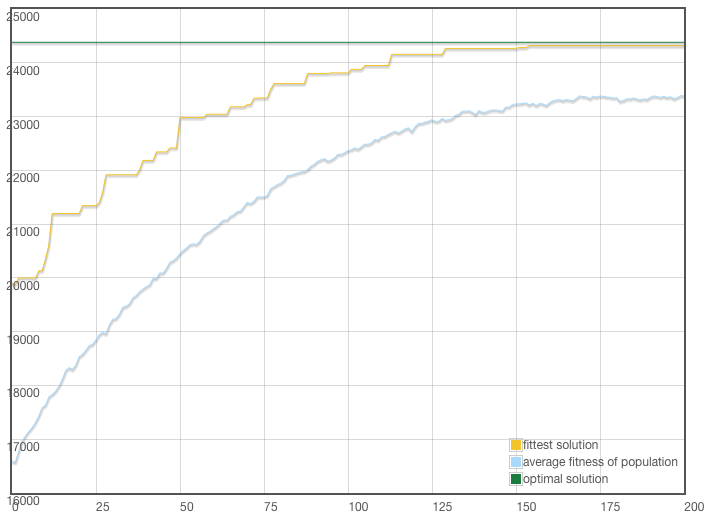
\includegraphics[width=0.9\textwidth]{images/convergence-p0.png}
\caption{Problem 0: convergence over generations}
\label{fig:convergence-p0}
\end{figure}
\end{center}

\subsection{Impact of parameters}

The tables analysing the impact\footnote{Computational time is based on a MacBook Air, i7 1.7 GhZ, Safari 7.0.4} of the change of a single parameter are based, except for the changed parameter, on the parameters in table \ref{tab:default}.

\begin{table}[h t b p]
\begin{center}
\begin{tabular}{ l | r }
parameter & value \\
\hline
max. generations 		& 200	\\
population size 		& 1000	\\
crossover probability	& 0.8	\\
mutation probability	& 0.3	\\
replace-worst proportion& 0.5	
\end{tabular}
\caption{Default parameters for the analysis}
\label{tab:default}
\end{center}
\end{table}

Table \ref{tab:maxgen} shows that the computation time is linearly increasing by the number of generations. This is also intuitively understandable. The quality of the solution is as well increasing, however not linearly. In the beginning at 10 to 90 generations the increase in fitness is apparent. After that it starts to slow down before it begins to converge at about 170.

\begin{table}[h t b p]
\begin{center}
\begin{tabular}{ l | l | r | r | r | r | r | r | r | r }
prob. & max. generations & 10 & 50 & 90 & 130 & 170 & 210 \\
\hline
\#0  & fittest solution	& 20287 & 22834 & 23899 & 24141 & 24304 & 24312 \\
& 	comp. time [ms]	  	& 563 & 2289 & 4211 & 6023 & 8014 & 10367 \\
\hline
\#29 & fittest solution	& 54575 & 57938 & 59167 & 59556 & 59878 & 59933 \\
& 	comp. time [ms]	  	& 465 & 2227 & 4097 & 6021 & 7847 & 10133 \\
\end{tabular}
\caption{Impact of max. generations parameter}
\label{tab:maxgen}
\end{center}
\end{table}

Population size showed to have a very large impact on computation time. Table \ref{tab:population} shows that it behaves nearly linearly from 200 to 1000. However, a size of over 1000 shows the limitations of the JavaScript implementation, as the computation time more than tripled. Below 100 we have an almost constant time behaviour, as the basic computation effort has a larger proportion than the population size. The fitness quality profits mainly in the range from 10 to 800. Higher values are slightly improving the quality. This also shows, that a too small population size limits the exploration of the search space.
   
\begin{table}[h t b p]
\begin{center}
\begin{tabular}{ l | l | r | r | r | r | r | r | r | r }
prob. & population size & 10 & 100 & 200 & 400 & 800 & 1000 & 2000 \\
\hline
\#0  & fittest solution	& 20374 & 23426 & 23779 & 23962 & 24253 & 24282 & 24326 \\
& 	comp. time [ms]	  	& 1672 & 1841 & 2361 & 3699 & 7279 & 9668 & 33333 \\
\hline
\#29 & fittest solution	& 56640 & 59708 & 59668 & 59756 & 59926 & 59896 & 59945 \\
& 	comp. time [ms]	  	& 1685 & 1914 & 2502 & 3766 & 7419 & 9499 & 30029 \\
\end{tabular}
\caption{Impact of population size parameter}
\label{tab:population}
\end{center}
\end{table}

Table \ref{tab:crossover} illustrates the importance of crossover. If no crossover happens, the quality is very low. Even just a probability of 0.1 improves the result a lot. This seems reasonable, as the crossover is a crucial part of the genetic algorithm idea. A probability of 0.4 to 1 showed the best results. The computation time is highly affected in the range from 0 to 0.1. This is due to population restrictions and the roulette wheel selection. If no crossover is performed, the offspring of the selected parents are plain copies. Additionally, the same parents are more often selected, caused by the roulette wheel. This leads to a very high chance of duplicated solutions which are rejected. Finally this leads to a long running loop until the population is filled. So the lower the crossover probability the higher the chance of duplicates.

\begin{table}[h t b p]
\begin{center}
\begin{tabular}{ l | l | r | r | r | r | r | r | r | r }
prob. & crossover prob. & 0 & 0.1 & 0.2 & 0.4 & 0.6 & 0.8 & 1 \\
\hline
\#0  & fittest solution	& 19929 & 23974 & 23998 & 24252 & 24235 & 24248 & 24381 \\
& 	comp. time [ms]	  	& 34090 & 12125 & 11236 & 9991 & 9793 & 9188 & 9145 \\
\hline
\#29 & fittest solution	& 48708 & 59563 & 59799 & 59896 & 59960 & 59955 & 59926 \\
& 	comp. time [ms]	  	& 34670 & 12377 & 11260 & 9844 & 9801 & 9406 & 9380 \\
\end{tabular}
\caption{Impact of crossover probability parameter}
\label{tab:crossover}
\end{center}
\end{table}

Mutation showed no significant impact on computation time (see table \ref{tab:mutation}). The quality of the solutions are best for 0.1 and 0.6 for problem 0. Problem 29 profits as well from low values in the range from 0 to 0.4. As only a single bit is flipped, the impact is not very large. By flipping sequences of bits the impact might be increased. 

\begin{table}[h t b p]
\begin{center}
\begin{tabular}{ l | l | r | r | r | r | r | r | r | r }
prob. & mutation prob. & 0 & 0.1 & 0.2 & 0.4 & 0.6 & 0.8 & 1 \\
\hline
\#0  & fittest solution	& 24179 & 24291 & 24202 & 24213 & 24312 & 24180 & 24231 \\
& 	comp. time [ms]	  	& 9027 & 9202 & 9435 & 9516 & 9591 & 9540 & 9702 \\
\hline
\#29 & fitness solution	& 59926 & 59892 & 59896 & 59906 & 59817 & 59852 & 59642 \\
& 	comp. time [ms]	  	& 9446 & 9778 & 9678 & 9344 & 9075 & 9526 & 9106 \\
\end{tabular}
\caption{Impact of mutation probability parameter}
\label{tab:mutation}
\end{center}
\end{table}

The proportion of the worst population which is replaced by the offspring has a large impact on the quality (table \ref{tab:crossover}). If it is too low (less than 0.2) not enough offspring can contribute to the population, so the diversity of the population stays low, which results in a poor performance which is mainly subject to the initial population quality. A too high value (more than 0.8) replaces very good solutions by probably less good offspring and therefore does not apply the principle \emph{survival of the fittest}. Values between 0.4 and 0.8 showed the best results. 

Computation time is also affected. It is increasing up to 0.8. This is due to  the additional effort to compute the offspring of a population. For a low value, only a few solution parents have to be selected and crossed which is faster than computing all. The slight drop for a proportion of 1 must be a outlier, maybe caused by the JavaScript runtime or tolerances in time measurement.

\begin{table}[h t b p]
\begin{center}
\begin{tabular}{ l | l | r | r | r | r | r | r | r | r }
prob. & replace proportion & 0 & 0.1 & 0.2 & 0.4 & 0.6 & 0.8 & 1 \\
\hline
\#0  & fittest solution	& 20276 & 22631 & 23606 & 24019 & 24138 & 24274 & 21552 \\
& 	comp. time [ms]	  	& 4124 & 5052 & 6059 & 9102 & 12856 & 14681 & 13044 \\
\hline
\#29 & fittest solution	& 50253 & 58236 & 59303 & 59942 & 59863 & 59955 & 54866 \\
& 	comp. time [ms]	  	& 4910 & 5638 & 6124 & 8560 & 11100 & 12112 & 12498 \\
\end{tabular}
\caption{Impact of replace-worst proportion parameter}
\label{tab:replaceworst}
\end{center}
\end{table}

Figure \ref{fig:impact} shows the overall impact of the parameters on the fittest solution and computation time. For that, the largest difference between the minimum and maximum of fitness and computation time for both problems have been calculated. Then the average of both is taken. This is repeated for each parameter.

\begin{figure}
\subfigure[fittest solution]{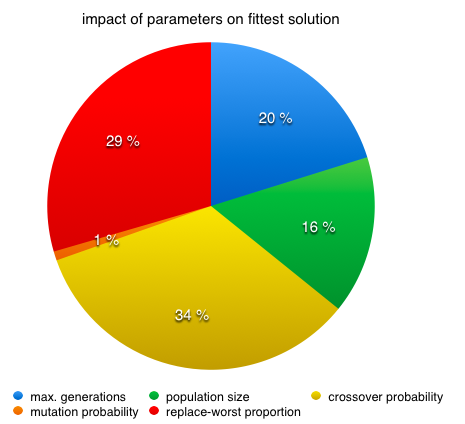
\includegraphics[width=0.49\textwidth]{images/impact-fittest.png}}\hfill
\subfigure[computation time]{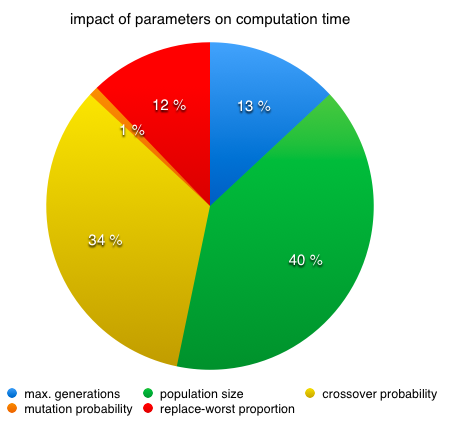
\includegraphics[width=0.49\textwidth]{images/impact-comptime.png}}
\caption{Impact of parameters on fittest solution and computation time}
\label{fig:impact}
\end{figure}


\section{Improvements}

\cite{bib:dj} suggests that the computation time and quality of the best solutions can be significantly increased by optimizing the initial population and applying penalty functions to infeasible solutions. 

By using the Dantzig algorithm a solution is found by considering the profit/weight ratio \(p_{i}/w{_i}\), i = 1 .. n.  Filling the knapsack is then done in a greedy way: Select the item with the largest p/w ratio and pack it in until the knapsack is filled and the constraint is met. In the mentioned multidimensional knapsack all constraints have to be considered. Applying this to the proposed algorithm could help to ensure a better quality of the initial population. As seen in the benchmarks, the initial population is poor and therefore needs some generations to gain quality. This could be overcome by using the Dantzig approach. However, it must be also checked that it does not lead to getting trapped in local maxima.

The penalty function drives invalid solution to valid ones and considers the profit of these solutions. The applying of the penalty is made in a proportion to the profit by considering the weight of a item which contributes to the violation of a constraint. This may improve the proposed GA in terms of computation time. As outlined in the benchmarks section, a large proportion of time is spent on evaluating and replacing invalid solutions after the crossover step, which could be improved by the penalty function. The convergence speed would also benefit from this, as the penalty function transforms invalid solutions to quite good solutions with high speed. It could also improve the quality, as the overall fitness of the population increases which therefore leads to a higher chance of better offspring.


\begin{thebibliography}{9}

\bibitem{bib:dj}
  Djannaty, F., Doostdar, S.,
  \emph{A Hybrid Genetic Algorithm
for the Multidimensional Knapsack Problem}.
  http://www.m-hikari.com/ijcms-password2008/9-12-2008/djannatyIJCMS9-12-2008.pdf,
  2008

\end{thebibliography}



\end{document}